		\documentclass[10pt,a4paper]{book}
		\usepackage[latin1]{inputenc}
		\usepackage{amsmath}
		\usepackage{amsfonts}
		\usepackage{amssymb}
		\usepackage{graphicx}
		\usepackage{float}
		\usepackage{hyperref}
		\hypersetup{
			colorlinks,
			citecolor=black,
			filecolor=black,
			linkcolor=black,
			urlcolor=black
		}
	\DeclareMathOperator{\E}{\mathbb{E}}
		\begin{document}
			\tableofcontents
			\newpage
			\chapter{Base concepts}
			\section{Density}
			$\dfrac{\text{edges of graph g}}{\text{num edges complete graph with n nodes}}$
			\section{BFS}
			\begin{itemize}
				\item Each node has three states: unvisited, visited, explored
				\item When a node is visited all non-visited neighbours are added into a FIFO queque, then the node is set as explored
				\item First, the starting node is explored
				\item While the queque is not empty:
				\begin{enumerate}
					\item Pick the first node in the queque
					\item Visit the node
				\end{enumerate}
			\item Each time a node is inserted into the queue, we also associate to this node its parent
			\item Property of BFS in unweighted graphs: the nodes at level i in the BFS tree are also the nodes at distance i in the graph
			\item When the graph is undirected it also allow us to know if the graph is connected (check the bfs tree contains all the nodes)
			\item You can know also the connected components of the graph doing a BFS from the non visited nodes while all are not explored
			\item Time complexity: each edge is considered two times: one when an extreme is visited and another when the other extreme is visited
			
			\end{itemize}
			\section{DFS}
			\begin{itemize}
				\item Same of BFS but instead of a FIFO queque use a LIFO queque or recursion
				\item Property of DFS: the dfs not include only the edges that link a node \textit{x} to its ancestor
				\item With the latter property we can use the DFS to check if a graph g contains a cycle
			\end{itemize}
			\section{Terms}
			\subsection{Subgraph}
			Subset of nodes of a graph g and all edges that links these nodes
			\subsection{Connected components}
			Maximal subgraph contained in the graph g where cannot be inserted more nodes
			\subsection{Graph connected}
		 A graph is connected if exists only one connected component
		 \subsection{Strongly connected components (direct graph)}
		 A direct graph is strongly connected contains only one maximal subgraph where exists a path from x to y \textit{and} from y to x
			\chapter{Algorithm for SCC in a direct graph}
			The problem is that when we perform the DFSs we can visit different connected components.
			\section{DAG}
			A DAG is a Directed Acyclic Graph. To check if a graph is a DAG with a DFS (see above).\\
			\section{Topologicals ordering}
			With a DAG you can sort the nodes in a \textit{topological ordering} with some alters to the DFS algorithm: 
			\begin{itemize}
				\item 	We denote as s(x) the time when a node x is visited and as f(x) the time when the invocation of dfs on the node ends
				\item When a node is visited the time indicator is increased and the the invocation ends the \textit{time} counter is increased then assigned as finished time
				\item At the end we can sort the nodes by finishing time
				\item If all nodes are not reached, remove all the reached nodes from the graph and then start a new DFS while all nodes are not removed
			\end{itemize}
			We demonstrate the following property: given a DAG, if exists an edge between a pair of nodes x and y $ (x \rightarrow y)  $ then $  f(x) > f(y) $:\\
			There are two possible option when the DFS is invoked with argument x: 
			\begin{enumerate}
				\item y is explored or y is not visited, otherwise is an ancestor edge but this not respect the hypotheses that g is a DAG. In the first case y is yet explored so it have assigned the  finished time while x not so is surely more than f(y).
				\item In the second case x is visited but the finished time is assigned after all the neighbours are explored (included y) so we return to the latter case
			\end{enumerate}
			\section{Component Graph}
			A component graph is a graph where the nodes are the SCC (strongly connected components) of g and exists an edge between $ c_1 $ and $ c_2 $ if exists one of the two options:
			\begin{itemize}
				\item exists an edge from a node in $ c_1 $ to $ c_2 $
				\item exists an edge from a node in $ c_2 $ to $ c_1 $
			\end{itemize}
			Any component graph is a DAG: for absurd if exists a bidirectional edge between $ c_1 $ and $ c_2 $ so the two nodes are not maximal so $ c_1 $ and $ c_2 $ should be an unique node
			\section{Graph transpose}
			The transpose $ G^T $ of a graph G is a graph where the edge directions are inverted. E.G. $ (a,b) \in G \rightarrow (b,a) \in G^T $
			\section{Kosaraju-Sharir algorithm}
			Base intuition: if we start the DFS in the last SCC of component graph (the SCC with only entering edge) then the DFS tree will include only the nodes of the SCC. Then remove the explored nodes from the graph and restart the DFS until all nodes are removed.\\
			Problem: We don't know the SCCs, that is what we want to find!\\
			Let's give some definitions:
			\begin{itemize}
				\item \textit{$ f(c) $}: largest finished time of a node in a connected component \textit{c}
				\item \textit{$ s(c) $}: smallest finished time of a node in a connected component \textit{c}
			\end{itemize}
			Let's prove the following assert: given $ c_1 $ and $ c_2 $ two connected components such as exists the edge $ (u,v) $ where $ u \in c_1 $ and $ v \in c_2 $, then $ f(c_1) > f(c_2) $.
			\subsection{Demonstration}
			We distinguish two cases:
			\begin{itemize}
				\item $ s(c_1) < s(c_2) $: Given \textit{x} the first node explored in $ c_1  $ then the DFS will find the edge $ (u,v) $ where $ u \in c_1 $ and $ v \in c_2 $ that continue the DFS in $ c_2 $. So it's obvious that for, how works the DFS and how are assigned the finishing times, the finishing time are first assigned to $ c_2 $ because the recursive calls through nodes in $ c_2 $ ends until reaches the node $ v $ that continue the assignment of the finishing time in $ c_1 $.\\
				In conclusion we can infer the following dis-equation:
				\begin{center}
				$ f(x) = f(c_1) > f(u) > f(v)  = f(c_2) $
				\end{center}
				\item $ s(c_1) > s(c_2) $: In this case we start in $ c_2 $ but we can infer that not exists a path  from $c_2$ to $ c_1 $ because the component graph is a DAG and exists for hypothesis the edge $ (u,v) $ where $ u \in c_1 $ and $ v \in c_2 $. So we can assert that the current DFS will not explore $ c_1 $ but a successive DFS will explore $ c_1 $ so $ f(c_1) > f(c_2) $
			\end{itemize}
			So we have demonstrate the latter assert.\\
		 From this proposition we can infer that if we take the node with the largest finished time we are surely in a SCC with only outgoing edges in the component graph! So if we do a DFS in the transpose graph we explore only the nodes in its connected component.\\
		 In conclusion the Kosaraju-Sharir algorithm is the following:
		 \begin{enumerate}
			 	\item Do DFS until all nodes have finishing time
			 	\item Transpose the graph
			 	\item Do DFS starting from the node with largest finishing. This is a connected component
			 	\item Remove all node explored
			 	\item Go to 3 until the graph have at least one node
		 \end{enumerate}
		 	Complexity: $ O(m) $
		 	\section{CC in social networks}
		 	\subsection{Giant component}
		 	A giant  component is a (strongly) connected component that contains a constant fraction of the nodes
		 	\subsection{Giant components in SN}
		 	The giant components is SN are very commons. \\
		 	In the web directed graph a common phenomenon is the \textit{bowtie phenomenon}: it says that we can classify the nodes in the following groups:
		 	\begin{itemize}
		 		\item \textit{SCC}: Nodes contained in a big giant strongly connected component
		 		\item \textit{IN}: the set of nodes that can only reach the \textit{SCC}
		 		\item \textit{OUT}: the set of nodes that can be reached from the \textit{SCC}
		 		\item \textit{tendrils}: nodes that can be reached only from \textit{IN} but are not part of \textit{SCC} and nodes that can reach \textit{OUT} but they are not part of \textit{SCC}
		 		\item \textit{disconnected}: nodes that can't reach the \textit{SCC} also if the graph is undirected
		 	\end{itemize}
		 	\section{Shortest path}
		 	In the case of undirected edges, the shortest path between two nodes x and y  is the minimum numbers of edges needed to reach y from x. It can be computed performing a BFS starting from x.\\
		 	There are two variants of this problem:
		 	\begin{itemize}
		 		\item SSSP (Single Source Shortest Path) that consists to find all the shortest path from a specific source
		 		\item APSP (All Pairs Shortest Path) that consists in find all the shortest path between all the pairs of nodes
		 	\end{itemize}
	 \chapter{Dijkstra's algorithm}
	 The Dijkstra's algorithm solves the SSSP problem in the case of weighted edges when the weights are positive. It is a \textit{greedy} algorithm, so it take the best decision only considering the current state and not the overall procedure.\\
	 At the beginning choose a starting node \textit{s} and then initialize a distance array $ dist $ with $ dist[s] = 0 $ and $ dist[x]  = \infty \,\, \forall x \neq s $ \\
	 The greedy step computed by Dijkstra is the following:
	 \begin{enumerate}
		 	\item choose a node \textit{x} not yet picked and that has the minimum $ dist[x] $
		 	\item for each neighbour $ y \in N(x) $ set $ dist[y] = \min(dist[y], \,\,dist[x] + d(x,y)) $
	 \end{enumerate}
		\section{Demonstration of the correctness of  Dijkstra's algorithm}
		To demonstrate the Dijkstra's algorithm we have to prove that given \textit{x} the node chosen at the step \textit{i} then $ dist[x] $ must be the minimum from \textit{s} to \textit{x}.\\
			Let's introduce some terms: $ A_i $ is the set of nodes picked at the step \textit{i} and $ d_i(x) $ the shortest path only through the nodes in $ A_i $.\\
			First, we prove by induction that $ dist[x] $ at the step i is equal to $ d_i(x) $:
			\begin{itemize}
				\item \textit{base case (i = 1)}  this case is simple: the shortest path from s to the neighbours $ y $ is simply $ d(s, y) = d_1(y) $
				\item \textit{inductive step} $ (k \rightarrow k+1) $ Let's suppose that the proof is valid until k so we have that $ dist[x] = d_k(n) \,\, \forall n \in A_k $. Given \textit{x} the node picked at the step k+1 and $ \pi_{k+1}(y) $ the shortest path from s to y through the nodes in $ A_{k+1} = A_k  \cup \{x\}$, for each edge $ (x, y) $ we have the two following cases about y:
				\begin{itemize}
					\item $ x \notin\pi_{k+1}(y)  $ it means that x is not in the shortest path from s to y not pass through x so we have that $ \pi_{k}(y)  = \pi_{k+1}(y)  $
					\item $ x \in\pi_{k+1}(y)  $  it means that the shortest path to y pass through x so we have that $ d_{k+1}(y) = d_k(x) + w(x,y) $
				\end{itemize}
			\end{itemize}
		Now we show that \textit{if x is the node chosen at the step i, a shortest path from s to x pass only through $ A_i $}.
		We demonstrate for absurd, so given \textit{y} the first node not in $ A_i $ that is in the shortest path of $ x  $ from $ s $ we can infer the following propositions:
		\begin{itemize}
			\item Since Dijkstra choose the node with minimum distance, $ d_i(x) =  dist[x]  \leq dist[y] = d_i(y) $
			\item $ d(s,y) < d(s,x) $ because all weights are positive and y is in the shortest path of x
			\item $ d(s,x) < d_i(x) $ since we are assuming that a shortest path from s to x not pass through nodes in $ A_i $
		 	\item  $ d(s,y) = d_i(y) $	since y is the first node outside of $ A_i $ (see above demonstration)
	\end{itemize}
	With the latter propositions we have an absurd because:\\ $ d(s,y) < d(s,x) < d_i(x) \leq d_i(y) = d(s,y) $\\
	\section{Complexity of Dijkstra's algorithm}
	The complexity depends on the data structure used to represent $ dist $.\\
	There are three types of time which complexity of Dijkstra's algorithm depends on:
	\begin{itemize}
		\item $ t_i $: The time to initialize $ dist $
		\item $ t_m $ Time to find the minimum in $ dist $
		\item $ t_u $ Time to update a value in $ dist $
	\end{itemize}
	Suppose that $ dist $ is an array, we have that:
	\begin{itemize}
		\item $ t_i = O(n) $ (Initialize $ n $ values) 
		\item $ t_m  = O(n)$ (Sequential search)
		\item $ t_u  = O(1)$ (Set a value in an array is immediate)
	\end{itemize}
		so the time complexity of Dijkstra's algorithm is 
		\begin{center}
			$ O(t_i + n t_m + m t_u)  = O(n + n\cdot n + m) = O(n^2) $ 
		\end{center}
		But if $ dist $ is an heap we have:
		\begin{itemize}
		\item $ t_i = O(n \log(n)) $ (Initialize $ n $ values and sort by heap property) 
		\item $ t_m  = O(\log(n))$ (Thanks to heap property)
		\item $ t_u  = O(\log(n))$ (Check heap property)
		\end{itemize}
		in this case the time complexity of Dijkstra's algorithm is 
		\begin{center}
			$ O(t_i + n t_m + m t_u)  = O(n \log(n)+ n \log(n) + m \log(n)) = O((n+m) \log(n)) $ 
		\end{center}
		which is good if the graph is sparse
		\chapter{Floyd-Warshall algorithm}
		This algorithm solve the APSP problem with  edges having negative edges, but that not contains a negative cycle because if it exists the shortest path should pass through the cycle infinitely.
		\section{Dynamic programming technique}
		The dynamic programming technique is used in the Floyd-Warshall algorithm and consists of saving in a data structure the results of sub-problems of a generic algorithm to use them when a call with the same input happens.
		\begin{figure}
			\centering
			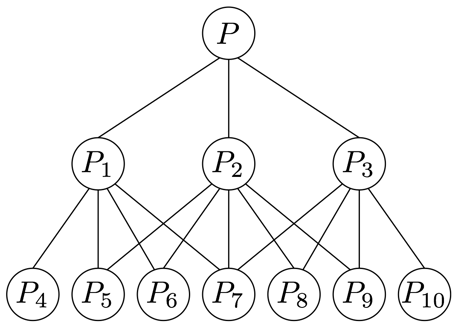
\includegraphics[width=0.5\linewidth]{img/DeepinScreenshot_20180222212118}
			\caption{Problem tree representation when it's useful the dynamic programming technique}
			\label{fig:deepinscreenshot20180222212118}
		\end{figure}
		\section{The algorithm}
		Let's define the following terms:
		\begin{itemize}
			\item $ A_0 = \emptyset $ and $ A_i = \{1 \dots i \} $
			\item $ \pi_i(x,y) $ the shortest path from x to y through the nodes contained in $ A_i $ (if x cannot reach y through $ A_i $ then $  \pi_i(x,y) = \infty $ )
			\item  $ d_i(x,y) $ the length of $ \pi_i(x,y) $
			\item Note that for $ i = 0 $ we have $ d_0(x,y) = w(x,y) $ if exists an edge between x and y else $ \infty $
		\end{itemize}
		For $ 1 \leq i \leq n $ we can calculate $ d_i(x,y) $ by distinguish between the two following cases:
		\begin{itemize}
			\item $ d_i(x,y)  $ pass through $ A_i $ but not by \textit{i}: in this case $ d_i(x,y) = d_{i-1}(x,y) $
			\item $ d_i(x,y)  $ pass through $ A_i $ and by \textit{i}: in this case $ d_i(x,y) = d_{i-1}(x,i) + d_{i-1}(i, y) $
		\end{itemize}
	\subsection{Complexity}
	\subsubsection{Space}
	This algorithm need a tri-dimensional array $ dist $ where the first dimension is used to memorize each step and the other two as matrix of the distance so the space complexity is $ O(n^3) $ but it can save some space memorizing only two matrix: the matrix of distances at step $ i $ and $ i-1 $, then the space complexity is $ O(n^2) $
	\subsubsection{Time}
	The time complexity is $ O(n^3) $ because for \textit{n} times the algorithm must update the distance matrix ($ O(n^2) $)
	\chapter{Six degree of separation}
	\section{The experiment}
	An experiment conducted by \textit{Stanley Milgram} says that, in 1990, the average distance between two persons in 6. He give to 296 people a letter that must be sent to the recipient and they can do two things:
	\begin{itemize}
		\item if it know the recipient: send directly the letter
		\item if it don't know the recipient: send the letter to the most probable person that maybe know the recipient
	\end{itemize}
	64 of 296 letters are delivered to the recipient and the average distance between the sender and the recipient is measured to be 6
	\section{Small world hypothesis}
	The experiment of \textit{Stanley Milgram} aims to verify that is called in SNA the \textit{small world hypothesis}, that means calculate the average shortest path across a network. In a social network, the average shortest path means calculate APSP (All Pair Shortest Path) then computationally is very often prohibitive (at least $ O(n^2) $ and in the worst case $ O(n^3) $).\\
	To avoid the high cost, we calculate an approximation of average shortest path using a \textit{sample} of nodes, but we need to measure the error of this approximation in order to use it rightfully.\\
	\section{Approximation of average shortest path}
	\subsection{Markov's inequality}
	The Markov's inequality is:
	\begin{center}
	$ Pr \left[ X \geq t \right] \leq \dfrac{\E\left[ X \right]}{t}$
	\end{center}
	The demonstration is simple:
	\begin{align*}
		 \E[X] &= \sum_u u \cdot P(X = u) \\
		 & \geq \sum_{u \geq t} u \cdot P(X = u)  \\
		  &\geq t \cdot \sum_{u \geq t}  P(X = u) = t\cdot P(X \geq t)  
	\end{align*}
	\subsection{The Chernoff's bounding method}
	 The Chernoff?s bounding method says that if X is a random variable and $ \forall t > 0 $ we can assert:
		\begin{center}
			$ P(X \geq t) \leq \min_{s > 0} e^{-st} \E\left[ e^{sX} \right]$
		\end{center}
		Using the Markov's inequality we can demonstrate the Chernoff?s bounding method:
		\begin{align*}
			P(X \geq t) &= P(sX \geq st)  \\
			&= P(e^{sX}\geq e^{st}) \leq e^{-st} \E \left[ e^{sX} \right]
		\end{align*}
		\subsection{Assert to demonstrate}
		If X is a random variable such that $ \E \left[ X \right] = 0 $ and $ a \leq X  \leq b $, for any $ s > 0 $ we have that:\\
		\begin{align*}
		\E \left[ e^{sX} \right] \leq e^{\dfrac{s^2(b-a)^2}{8}}
		\end{align*}
		Since $ e^{sx} $ is convex we have that:
		\begin{align*}
			e^{sX} \leq \dfrac{X -a }{b-a} e^{sb} + \dfrac{b-X}{b-a} e^{sa} 
 		\end{align*}
 		For hypothesis $ \E \left[X\right]  = 0$ so we have that:\\
 		\begin{align*}
 		  \E \left[e^{sX} \right] &\leq  \E \left[ \dfrac{X -a }{b-a} e^{sb} + \dfrac{b-X}{b-a} e^{sa}  \right] \\
 		  &= -\dfrac{a }{b-a} e^{sb} + \dfrac{b}{b-a} e^{sa}
 		\end{align*}
 		Now we define $ p = \dfrac{b}{b-a} $ and $ u = s(b-a) $, then we rewrite the latter formula in a log  scale with the new terms:
 		\begin{align*}
 		 		\log \left(   \dfrac{b}{b-a} e^{sa}  -\dfrac{a }{b-a} e^{sb} \right) 
 		 				&= sa + \log \left(p + (1 - p)e^{s(b-a)}\right) \\
 		 		&= (p-1) u + \log(p+(1-p) e^u) = \varphi(u)
 		\end{align*}
 		
		We apply the Taylor theorem to $ \varphi(u) $:
\begin{align*}
\varphi(u) = \varphi(0) + \varphi'(0) u + \dfrac{1}{2} \varphi''(\xi)u^2
\end{align*}
Since $ \varphi(0) $ and $ \varphi'(0) $ are 0 and $ \varphi''(\xi)  \leq \dfrac{1}{4}$ we have that:\\
\begin{align*}
\varphi(u) &= \dfrac{1}{2} \varphi''(\xi)u^2 \\
&\leq \dfrac{u^2}{8} = \dfrac{s^2(b-a)^2}{8}
\end{align*}
		\subsection{The Hoeffding's inequality}
		Given k independent random variables $ X_1 \dots X_k $ such that $ a_i \leq X_i \leq b_i $ and $ X = \sum_i X_i $ for any $ t > 0 $ we have that:
		\begin{align*}
			P(X - \E\left[X\right] \geq T) \leq e^{\dfrac{-2t^2}{\sum_{i=1}^{k} (b_i - a_i)^2}}
		\end{align*}

		If we apply the \textit{Chernoff's bounding method} to $ X - \E \left[X\right] $ we have that \\
		\begin{align*}
			P(X - \E \left[ X\right]  \geq t)  &\leq \min_{s > 0} e^{-st} \E \left[ e^{s(X - \E \left[X\right])} \right] \\
			& =\min_{s > 0} e^{-st} \prod_{i=0}^{k} \E \left[ e^{s(X_i - \E \left[X_i\right])} \right] \\
			& = \min_{s > 0} e^{-st} \prod_{i=0}^{k} e^{\dfrac{s^2(b_i - a_i)^2}{8}} \\
			&=  \min_{s > 0}  e^{-st}  e^{\dfrac{s^2\sum_i (b_i - a_i)^2}{8}} \\
			&= \min_{s > 0} e^{-st + \dfrac{s^2\sum_i (b_i - a_i)^2}{8}}
		\end{align*}
		In conclusion we have that $ 	P(X - \E \left[ X\right]  \geq t)  \leq  \min_{s > 0} e^{-st + \dfrac{s^2\sum_i (b_i - a_i)^2}{8}} $.
		Now we want to minimize the exponent of e for the Hoeffding's inequality, so we derive $ -st + \dfrac{s^2\sum_i (b_i - a_i)^2}{8} $ by s and we obtain a minimum for $ s = \dfrac{4t}{\sum_{i=1}^{k}(b_i - a_i)^2} $ .
		If we substitute we have:
		\begin{align*}
		P(X - \E \left[ X\right]  \geq t) & \leq  \min_{s > 0} e^{-st + \dfrac{s^2\sum_i (b_i - a_i)^2}{8}} \\
		&= e^{-\dfrac{4t}{\sum_{i=1}^{k}(b_i - a_i)^2} \cdot t + \dfrac{\left(\dfrac{4t}{\sum_{i=1}^{k}(b_i - a_i)^2} \right)^2\sum_i (b_i - a_i)^2}{8}} \\
		&=e^{-\dfrac{4t^2}{\sum_{i=1}^{k}(b_i - a_i)^2} + \dfrac{\dfrac{\left(4t\right)^2}{\sum_{i=1}^{k}(b_i - a_i)^2} }{8}} \\
		&= e^{\dfrac{-4t^2 \cdot 8 + \dfrac{\left(4t\right)^2}{\sum_{i=1}^{k}(b_i - a_i)^2} \cdot \sum_{i=1}^{k}(b_i - a_i)^2 }{\sum_{i=1}^{k}(b_i - a_i)^2 \cdot 8}} \\
		&= e^{ \dfrac{(4t)^2(-2+1)}{ \sum_{i=1}^{k}(b_i - a_i)^2 \cdot 8} } \\
		&= e^{ - \dfrac{16t^2}{ \sum_{i=1}^{k}(b_i - a_i)^2 \cdot 8} } = e^{ - \dfrac{2t^2}{ \sum_{i=1}^{k}(b_i - a_i)^2} }
		\end{align*}
		
		The Hoeffding's inequality works also when random variables are in the form $ -X_1 \ldots -X_k $ because
		\begin{align*}
			P(X - \E\left[X\right] \leq -t) \leq e^{ - \dfrac{2t^2}{ \sum_{i=1}^{k}(b_i - a_i)^2} } \\
			P(|X - \E\left[X\right ]| \geq  t) \leq 2e^{ - \dfrac{2t^2}{ \sum_{i=1}^{k}(b_i - a_i)^2} } \\
		\end{align*}
		\section{Finally the approximation}
		We can define grthe average shortest path at distance h as
		\begin{align*}
			N_h = \dfrac{|\{ (u,v) \in V \times V : d(u,v) = h \}|}{n(n-1)}
		\end{align*}
		instead of V if we sample from V a subset  $ U = \{u_1 \ldots u_k \} \subseteq V $ we have
		\begin{align*}
			N_h(U) = \dfrac{|\{ (u,v) \in U \times V : d(u,v) = h \}|}{|U|(n-1)} = \dfrac{\sum_{i=0}^{k} N_h(\{u_i\})}{k}
		\end{align*}
		The expected value of $  N_h(\{u_i\}) $ is
		\begin{align*}
			\E \left[ N_h(\{u_i\})  \right]	&= \dfrac{1}{n} \sum_{v \in V} N_h(\{v\})   \\
			& = N_h(V) = N_h
		\end{align*}
		then the expected value of set $  U  \subseteq V$ is
		\begin{align*}
			\E \left[N_h(U)\right] &= \E \left[\dfrac{\sum_{i=1}^{k} N_h(\{u_i\})}{k}\right] \\
			&= \dfrac{\sum_{i=1}^{k} \E \left[ N_h(\{u_i\} \right])}{k} \\
			&= \dfrac{\sum_{i=1}^{k} N_h}{k} \\
			&= \dfrac{k N_h}{k} = N_h
		\end{align*}
		Because $ N_h $ is a ratio, we can assert that $ 0 \leq N_h \leq 1 $ so $ \forall \,\, i \,\, N_h(\{u_i\}) $ we can define $ a_i = 0 $ and $ b_i = 1 $. So we can apply the Hoeffding's inequality to $ N_h $ to obtain this approximation:
		\begin{align*}
		P\left( \lvert  \dfrac{\sum_{i=1}^{k}  N_h(\{u_i\} )}{k} - N_h \rvert \geq t \right) \leq   2e^{-2t/k}
		\end{align*}
		If we choose the sample size $ k = \frac{2}{\alpha}t^{2}  \dfrac{1}{\ln(n) }$ we obtain the following bound
		\begin{align*}
			2 e^{\dfrac{-2t^2 \ln(n)}{\frac{2}{\alpha}t^{2} }} &= 2 e^{ - \alpha \cdot \ln(n)}\\
			&= 2 e^{\ln(n^{ - \alpha})} \\
			&= 2 n^{ - \alpha}
		\end{align*}
		Then the upper bound is dependent from $ \alpha $ (often $ \alpha = 2 $)
		
		\chapter{Compute the diameter}
\section{Definition of diameter}
The diameter is the maximum distance between two vertices
\section{A simple approach}
In the general case the best approach is calculate APSP (All Pairs Shortest Path) then find the maximum distance, that has a time complexity of $ O(n^{2.38}) $ where the 2.38 derive from some optimization on matrix calculation(see below) for dense graph while $ O(mn) $ for sparse graph. The problem with this simple approach is that is not usable in real-world graphs because contains millions of nodes and edges.
\section{Lower bound for diameter computation}
\subsection{SETH Hypothesis}
The Strong Exponential Time Hypothesis (SETH) says that there not exists an algorithm that solves k-SAT in less than $ O((2-\epsilon)^n) $ where $ \epsilon > 0 $
\subsection{Reduction between two problems}
Given two problems A and B, the relative sets of instances of the problem $ I_A $ and $ I_B $ and the solutions set $ A(x) $ and $ B(x) $ of a instance $ x $ we can say that A is reducible to B if exists two functions \textit{f} and \textit{g} where given $ x \in I_A $, $ x' = f(x) \in I_B $, $ y' = B(x') $ and $ g(y', x) \in A(x) $

\begin{figure}[H]
	\centering
	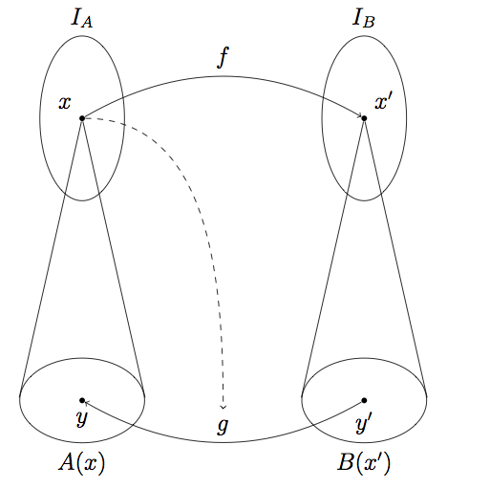
\includegraphics[width=0.7\linewidth]{img/problem_reduction}
	\caption{Graphical representation of problem reduction}
	\label{fig:problemreduction}
\end{figure}
\subsection{K-SAT*}
A variant of the k-sat problem is the $ K-SAT^* $ where between them change only the input: The $ K-SAT^* $ receive two sets of assignments $ X  $ and $ Y$ of size $ n = 2^{\frac{m}{2}} $ to respectively the first half and second half of variables where m is the number of variables and a set of clauses $ C $.\\
In order to find an assignment that satisfy $ C $ we combine each first-half assignment of X to Y, then try to check if applied to the set of clauses returns \textit{true}.\\
So the complexity of the algorithm is virtually $ O(n^2) $ on the input size, but if we substitute n in function of m (the number of variables) we obtain $ O((2^{\frac{m}{2}})^2)  = O(2^m)$. Also this problem cannot have the complexity $ O(n^{2-\varepsilon}) $ unless SETH is false.
Remember that SAT clauses are in CNF form that means:\\ \medskip
\noindent
$ (X_{1}\vee X_{2}\vee \cdots \vee X_{n})\wedge (Y_{1}\vee X_{2}\vee \cdots \vee X_{n})\wedge (X_{1}\vee Y_{2}\vee \cdots \vee X_{n})\wedge (Y_{1}\vee Y_{2}\vee \cdots \vee X_{n})\wedge \cdots \wedge (Y_{1}\vee Y_{2}\vee \cdots \vee Y_{n}). $\\
To resume in words, in CNF  variables in the clause are concatenated with OR operator while the clauses are concatenated with AND operator
\subsection{Disjoint set problem}
Given a set of sets C, the solution is 1 when exists two sets $ A,B \in C $ such that $ A \cap B = \emptyset $.
The complexity of this algorithm is $ O(|C|^2) $.
\subsection{Reduction from K-SAT* to disjoint set}
Given the set of all clauses $ C $ and X,Y respectively the assignment to the first and second half of variables, we define the collection $ S = S_1 \cup S_2 $ as follow:
\begin{center}
	$ S_1:= \{ \{t_1\} \cup \{ c : x \in X \nvDash c \,\, \forall c \in C \} \}$ \\ \medskip
	$ S_2:= \{ \{t_2\} \cup \{ c : y \in Y \nvDash c \,\, \forall c \in C \} \}$
\end{center}
$ t_1 $ and $ t_2 $ are only tokens to avoid the empty intersection between set from the same assignment.\\
To resume, if exists a good assignment in $ K-SAT^* $ then in disjoint sets should exists an empty intersection between two sets, one in $ S_1 $ and another in $ S_2 $.\\
To explain the reduction from $ K-SAT^* $ to disjoin set, a good assignment should satisfy all the clauses in K-SAT* and this thing is transposed in disjoint set with the intersection operator: given $ s_1 \in S_1 $ and $ s_2 \in S_2 $ if $ s_1 \cap s_2 \ne \emptyset$ then exists a clause not satisfied both from X and Y so the clause if false, then is not a good assignment while a good assignment should satisfy all the clauses so it should not have any clause in the intersection.
\subsection{From disjoint set to diameter computation}
Given in input a set of sets $ C $ and the variables $ X $ we can build a clique of the size of  $ X $, then add a node for each subset in $ C $ and add an edge between the node  $ c_i \in C $  and $ x_j $ if $ x_j $ appears in the set $ c_i $.\\
Then we can interpreter the diameter between $ c_i \text{ and } c_j $ in the following mode :
\begin{itemize}
	\item $ diameter(c_i, c_j) = 2  \rightarrow $  exists an intersection between $ c_i $ and $ c_j $
	\item $ diameter(c_i, c_j) = 3  \rightarrow $ not exists an intersection between $ c_i $ and $ c_j $
\end{itemize}
\begin{figure}[H]
	\centering
	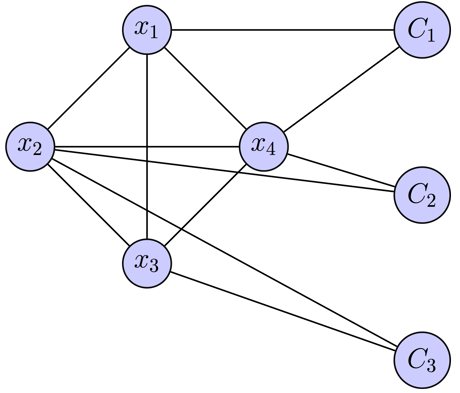
\includegraphics[width=0.5\linewidth]{img/disjoint_set_to_diameter}
	\caption{Graphical representation of reduction from disjoint sets to diameter computation}
	\label{fig:disjointsettodiameter}
\end{figure}
\subsection{Complexity of diameter computation}
With the above reductions we have demonstrated that the complexity of diameter computation cannot be in the form $ O(n^{2 - \varepsilon}) $ unless SETH is false, so the complexity of diameter cannot be lower than $ O(n^2)  $
\section{Heuristic for computing the diameter}
\subsection{BFS and diameter}
The height of BFS tree is a lower bound for computing the diameter. We can use this value also as approximation of the diameter doing many BFS from a random vertex. Below we present two methods to approximate the diameter with BFS. This approximations works well in various types of graphs (including social networks) but in other types not, for example road networks.
\subsection{2-SWEEP}
\begin{enumerate}
	\item Pick a random vertex \textit{r}
	\item Do a BFS from r
	\item Pick \textit{x}, one of the farther vertexes from r
	\item Do a BFS from \textit{x} and return the height of the BFS tree as diameter
\end{enumerate}
Complexity: $ 2 \cdot m $

\begin{figure}[H]
	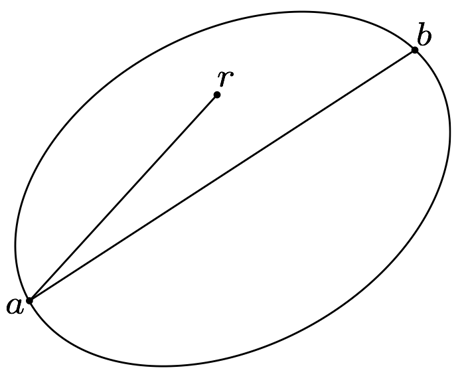
\includegraphics[width=0.4\linewidth]{img/2sweep}
	\caption{2-SWEEP graphical representation}
	\label{fig:2sweep}
\end{figure}
\subsection{4-SWEEP}
\begin{enumerate}
	\item Do a 2-SWEEP
	\item Pick one of the middle vertexes in the longest path of the 2-SWEEP
	\item Do a 2-SWEEP from that vertex
\end{enumerate}
Complexity: $ 4 \cdot m $
\section{Exact heuristic of diameter}
\subsection{Eccentricity}
The eccentricity of a vertex $ ecc(v) $ is the maximum distance between $ v $ and any other node
\subsection{}
		\chapter{Power law phenomenon}
\section{The power law}
Initially the simplest distribution assumed for the degree distribution on a social network is a \textit{Normal Gaussian}. But it is verified that the distribution of the degree is proportional to $ f(k) = \frac{1}{k^\beta} $ with $ \beta  $ close to 2. A function $ f(k) $ that decrease as increase $ k $ is called \textit{power law}
\subsection{Difference between a normal distribution and a power law}
The normal distribution is a representation of a balanced phenomenon, where in the mean there is the maximum frequency and in the slopes decrease the frequency.\\
In the power law instead is a representation of a imbalanced phenomenon where, with small values of x we have high frequency and with high values x we have a small frequency. Some example of power law phenomenon are the richness, number of relations in a social network.
\begin{figure}[H]
	\centering
	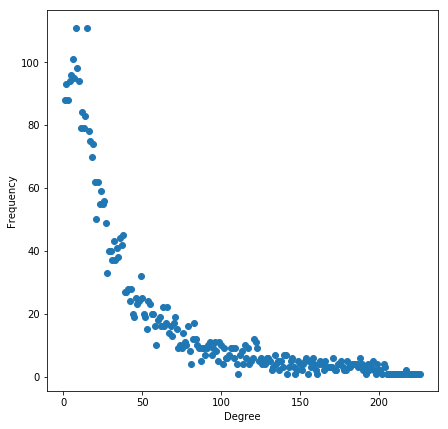
\includegraphics[width=0.7\linewidth]{img/power_law_example}
	\caption{Degree distribution on a Facebook social network}
	\label{fig:powerlawexample}
\end{figure}
\subsection{Check if a degree distribution is a power law}
In order to check if a degree distribution is a power law it must be in the form $ f(k) = \alpha \cdot \dfrac{1}{k^{\beta}} $.
We can do a linear regression in log-log scale of $ f(k) $ that is
\begin{align*}
\log(f(k)) = \log\left(\dfrac{\alpha}{k^{\beta}}\right) = \log(\alpha) - \beta \cdot \log(k)
\end{align*}
and should be a straight line to represent a power law

\section{Generative model of social network based on degree distributions}
In this section we study some generative models based on degree distribution of real graph. The generative models aim to estimate the $ p(x) $, the distribution of data that in this case is a social network
\subsection{Erd\"{o}s-Gilbert-R\'{e}nyi model}
This model is very simple, in fact it consider the probability \textit{p} that exists an edge between two nodes is independent to any other. \\ In statistical terms we can consider the distribution edge as a $ Bernoulli(k;p) $.\\ In this case we define the graph as $ G(n,p) $ where n is the number of nodes and p the probability that exists an edge.\\
The expected number of edges is:
%In prof handouts the formula is wrong, this is taken from https://economics.mit.edu/files/4621
\begin{align*}
\E \left[ Edges \right]= \sum_{1\leq x \leq y \leq n} (1\cdot p + 0 \cdot (1-p)) = \sum_{1\leq x \leq y \leq n} p = \binom{n}{2} p = \dfrac{n(n-1)}{2} p
\end{align*}
Since in a indirect graph an edge is present in the two extremes of the edge the expected degree of a node is $ 2 \cdot   \frac{n(n-1)}{2} p $.\\
The probability that a node have \textit{k} neighbours is a binomial distribution  so we can express as $ Bin(k; n, p) = \binom{n}{k} \cdot p^k \cdot (1-p) $. %also here an error on prof handouts 
\\
This model for \textit{n} and \textit{k} sufficiently big approximate to a normal distribution
\subsection{Chung-lu model}
In this model the probability that exists an edge between two nodes is proportional to the expected degree of the pair of nodes.
\begin{itemize}
	\item Initially we set $ \textbf{d} = (d_1 \ldots d_n) $, the expected degree of each node.
	\item The probability that exists an edge between the node \textit{i} and \textit{j} is \begin{align*}  p(E_{ij}) = \dfrac{d_i d_j}{\sum_k d_k} 	\end{align*} 
\end{itemize}
If the degree distribution \textbf{d} is a power law, then the graph generated is a power law
\subsection{Barabasi-Albert model}
The previous models are static, in fact they have a fixed number of nodes. \\This model is dynamic so it mean that doesn't require the number of nodes a priori but they can be added always.\\ 
With this dynamism try to give an explain to creation of a social network at difference of the previous models.\\
Every time a node is inserted an edge is created with the \textit{preferential attachment} system.
\subsubsection{Preferential attachment system}
Every time a node \textit{j} is added, a direct edge is created with the following two possibilities:
	\begin{itemize}
		\item with probability \textit{p} choose a random node $ i < j $  
		\item with probability $ (1-p) $ choose a node with probability proportional to the in-degree of the node
	\end{itemize}
The latter option is called \textit{rich-get-richer rule}. In fact if you have a  high number of relation you are more likely to make more.
\subsubsection{Degree distribution}
When a node \textit{j} is created, the probability that exists the edge $ (j, i)) $ with $ j > i $ is:
\begin{align*}
P(E_{ji}) &= \dfrac{1}{j-1} \cdot p + \dfrac{G_i(j-1)}{\sum_{h \leq (j-1)} G_h(j-1)} \cdot (1-p) \\
&=  \dfrac{1}{j-1} \cdot p + \dfrac{G_i(j-1)}{j-1} \cdot (1-p) 
\end{align*}
where $ G_i(j-1) $ is the in-degree of the node \textit{i} at the time $ j-1 $
\subsubsection{Deterministic $ G_j(t) $}
We want to find an approximation of $ G_j(t) $ that give deterministically the in-degree of a node $ l $ at time $ t $. Let us denote as $ g_l(t) $ the approximation of $ G_l(t) $. The increase of in-degree can be expressed from a differential equation:
\begin{align*}
	& \dfrac{d(g_l(t))}{dt} = \dfrac{p}{t} + \dfrac{ g_l(t) \cdot (1-p)}{t} = \dfrac{p + g_l(t) (1-p)}{t} \\
	& \dfrac{d(g_l(t))}{dt} \cdot \dfrac{1}{p + g_l(t) (1-p)} =  \dfrac{1}{t} \\
	& \int \dfrac{d(g_l(t))}{dt} \cdot \dfrac{1}{p + g_l(t) (1-p)} dt = \int   \dfrac{1}{t}  dt \\
	& g_l(t) \cdot \dfrac{\ln(p + g_l(t) (1-p))}{1-p} + c' = \ln(t) + c'' \\
	& g_l(t) \cdot  \ln(p + g_l(t) (1-p)) =  \ln(t) \cdot (1-p) + c \\
	& e^{\ln(p + g_l(t) (1-p))} = e^{\ln(t) \cdot (1-p) + c} \\
	&e^{\ln(p + g_l(t) (1-p))} = e^{\ln(t) \cdot (1-p) } \cdot e^c \\
	&(p + g_l(t) (1-p)) = t^{(1-p) } \cdot e^c \\
	& g_l(t) = \dfrac{t^{1-p} \cdot e^c - p}{1-p}	 
\end{align*}
When we insert the node $ l $ at time $ l $ we have that $ g_l(l) = 0  $ so we have
\begin{align*} 
 & 0= \dfrac{l^{1-p} \cdot e^c - p}{1-p}	 \\
 & \dfrac{p}{1-p} =\dfrac{l^{1-p} \cdot e^c}{1-p} \\
 &	e^c = \dfrac{p}{l^{1-p}}
\end{align*}
if we substitute the latter expression in $ g_l(t) $ we have
\begin{align*}
	 &g_l(t) = \dfrac{t^{1-p} \cdot \dfrac{p}{l^{1-p}} - p}{1-p}  \\
	 &g_l(t) = p \cdot \left( \left(\frac{t}{l}\right)^{(1-p)}  -1 \right) \cdot \dfrac{1}{1-p}
\end{align*}
\noindent
We can use the latter expression to estimate the number of nodes that at time \textit{t} have degree at least \textit{k}. So we write
\begin{align*}
	& \left( \left(\frac{t}{l}\right)^{(1-p)}  -1 \right) \cdot \dfrac{p}{1-p} \geq k \\\\
	&\text{Then we pone respect to l: } \\
	& \left(\frac{t}{l}\right)^{(1-p)} \geq k \cdot \dfrac{1-p}{p} + 1 \\
	& \frac{t}{l} \geq \left(k \cdot \dfrac{1-p}{p} + 1\right)^{\frac{1}{1-p}} 
	\end{align*}
Note that the next expression is the fraction of nodes at time \textit{t} that have at least in-degree \textit{k}:
\begin{align*}
	 & \frac{l}{t}\leq \left(k \cdot \dfrac{1-p}{p} + 1\right)^{-\frac{1}{1-p}} \\
	  & l \leq t \cdot \left(k\cdot \dfrac{1-p}{p} + 1\right)^{-\frac{1}{1-p}}
\end{align*}
To have the nodes that have \textit{exactly k in-degree} at \textit{time t} we must take the opposite of derivative (why?) of $  \left(k \cdot \dfrac{1-p}{p} + 1\right)^{-\frac{1}{1-p}} $ respect to k.\\ The result is 
\begin{center}
	$ \dfrac{1}{1-p} \left( k \dfrac{1-p}{p} + 1 \right)^{-\left(1 + \frac{1}{1-p}\right)} $
\end{center}
We can infer from the latter expression that the distribution of in-degree nodes is a power law with exponent $ \beta =  1 + \frac{1}{1-p}$.\\
From 
\begin{itemize}
	\item  when $ p \simeq 1 $ we exponent disappear then we tend to Erd\"{o}s-Gilbert-R\'{e}nyi model.
	\item when $ p \simeq 0 $ we apply almost ever the Preferential Attachment  System,  so the new nodes will more probably link to others with high in-degree, that is very similar to what happen with Chung-lu model.
	\item The distribution disappear when $ p \propto k^{-2} $ %Not understand how
%	in fact we have\\ $ \left( k \dfrac{1-k^{-2}}{k^{-2}} + 1 \right)^{-\dfrac{1-k^{-2}+1}{1-k^{-2}}}  = \left( k \dfrac{1-k^{-2} + k^{-2}}{k^{-2}} \right) ^ {\dfrac{k^{-2}-2}{1-k^{-2}}}= k^{3 \cdot \dfrac{k^{-2}-2}{1-k^{-2}}}$
\end{itemize}
		
	\end{document}	